\documentclass[12pt, english]{article}
\usepackage[utf8]{inputenc} %packages
\usepackage[T1]{fontenc}
\usepackage{babel}
\usepackage{listings}
\usepackage[text={20cm,25.5cm}]{geometry}
\looseness=-1
\usepackage[T1]{fontenc}
\usepackage{float}
\usepackage{graphicx}
\usepackage{caption}


\begin{document}
{\Large \textbf{Amit Sarker, Roll: 99}}
\section{\textit{Design of the solution}}
\par
I have generated a random graph \textit{(graph = nx.erdos\_renyi\_graph(N, P))} using \textit{networkx} library, where \textit{N = number of nodes}, \textit{P = probability}, which means \textit{each edge is included in the graph with probability P independent from every other edge}. From the graph, I have generated the variable, domain and constraint list. \textit{Domains} are randomly selected with a fixed length domain size and I have used 10 \textit{constraints} which are assigned randomly to every node as I described my earlier problem description assignment. I have used this graph for all the arc-consistency algorithms and the comparisons and findings are described in the following sections.

\section{\textit{Comparisons}}
\par
I have compared all these four algorithms (\textbf{AC-1}, \textbf{AC-2}, \textbf{AC-3}, and \textbf{AC-4}) based on \textit{\textbf{total number of nodes vs run time}} and \textit{\textbf{probability of edges vs run time}}. For both cases, I have changed the domain size from \textit{5 to 85}, increased by \textit{20}. I have calculated the average run time for each domain size. I have taken an average of \textit{200 iterations} for both cases to calculate the average run time. For comparing the \textit{total number of nodes vs run time}, I have changed the value of the total number of nodes from \textit{5 to 95}, increased by \textit{10}. I have fixed the probability of edge to \textit{0.5} for this case. For the second case, \textit{probability of edges vs run time}, I have changed the value of the probability of edge from \textit{0.1 to 0.9}, increased by \textit{0.1}. I have fixed the number of total nodes to \textit{20} for this case. The graphs are shown below:\\

\hspace*{0.5cm}$\bullet$ \textit{\textbf{Total number of nodes vs Run time:}}
\begin{figure}[ht]
		{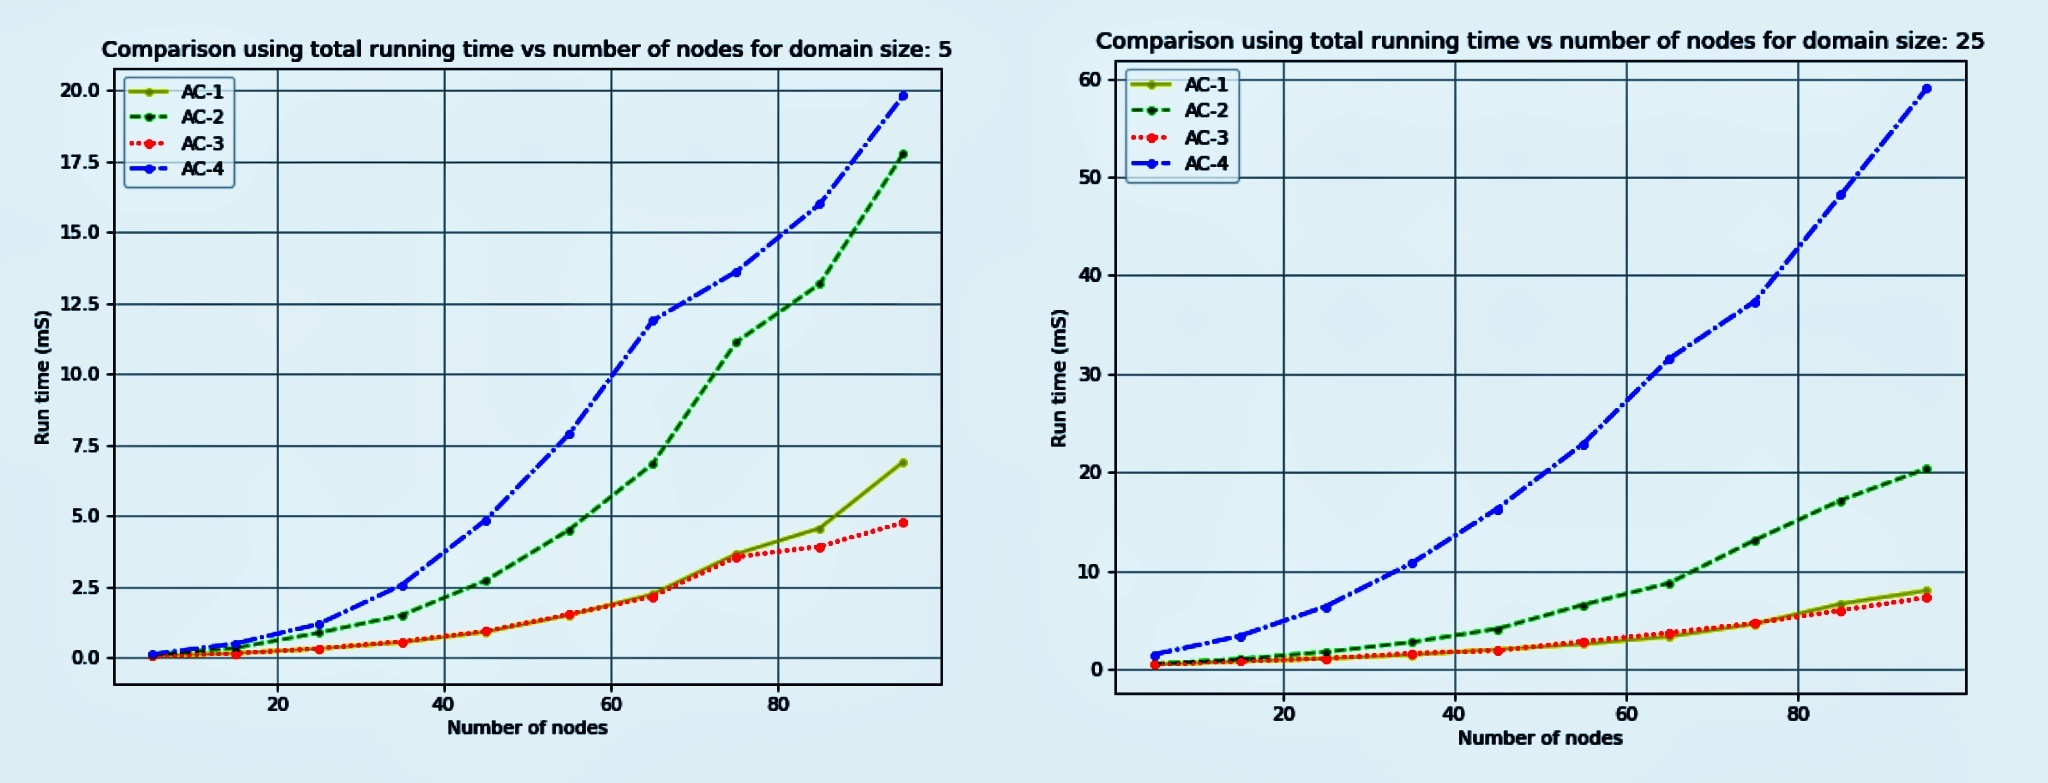
\includegraphics[width=\textwidth,height=2.6in]{11.jpeg}}
		{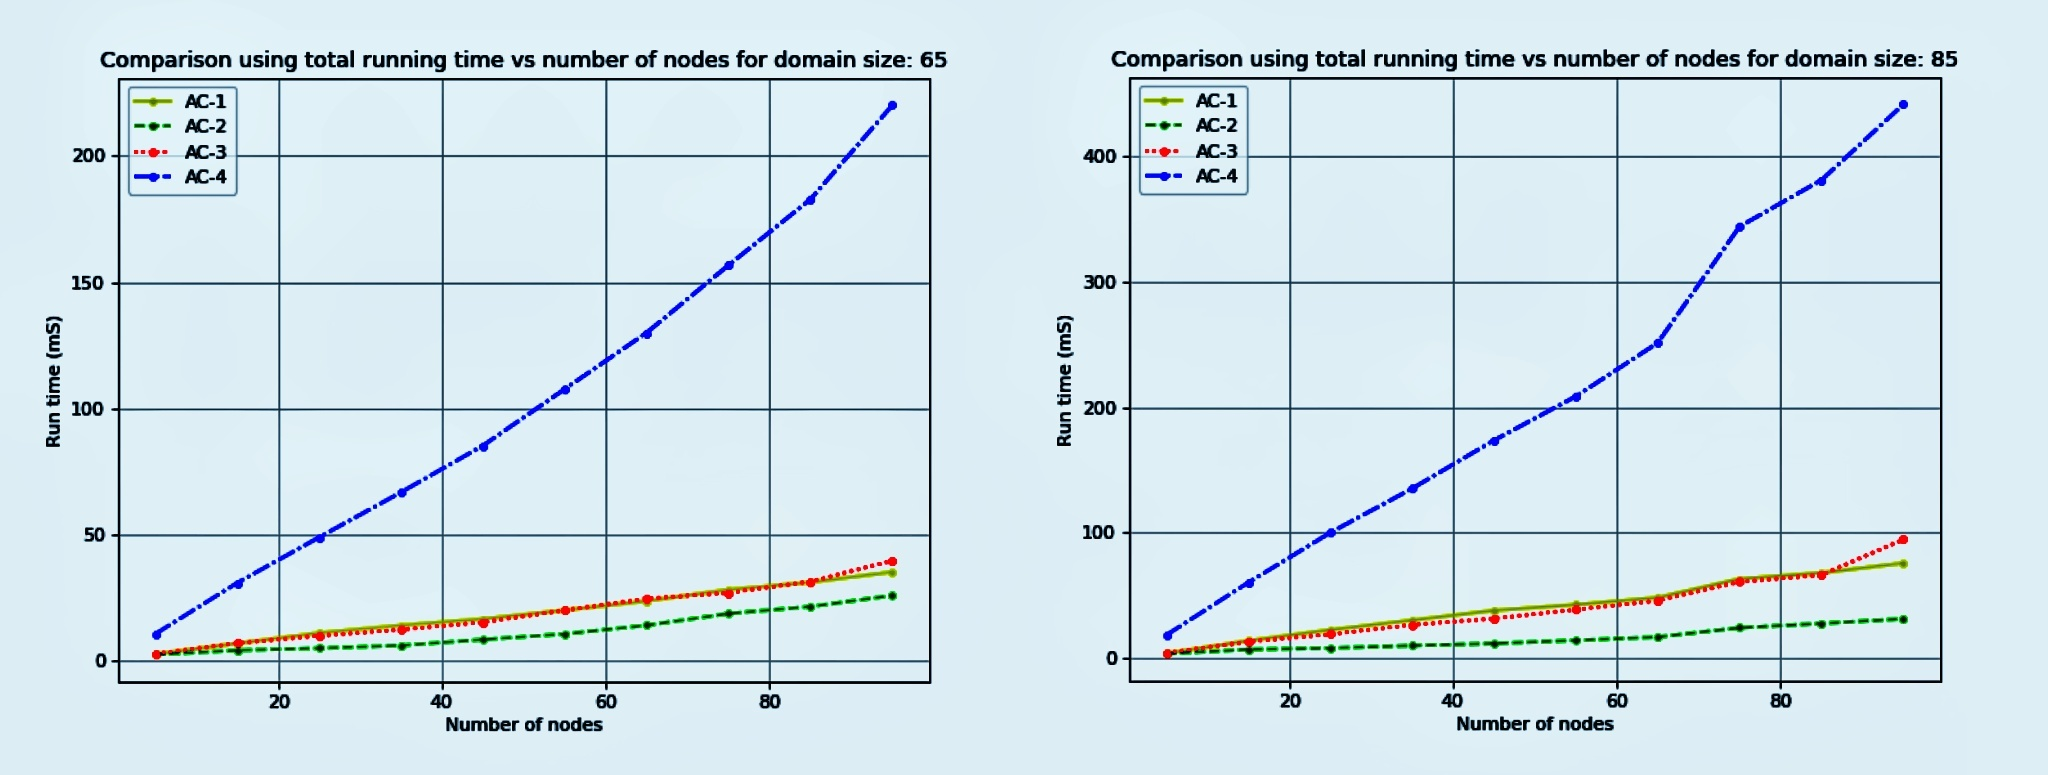
\includegraphics[width=\textwidth,height=2in]{22.jpeg}}
		\caption{\textbf{Total number of nodes vs Run-time for domain size 5, 25, 65, 85}}
        \label{fig: 1}
\end{figure}

\hspace*{0.5cm}$\bullet$ \textit{\textbf{Probability of edges vs Run time:}}
\begin{figure}[ht]
		{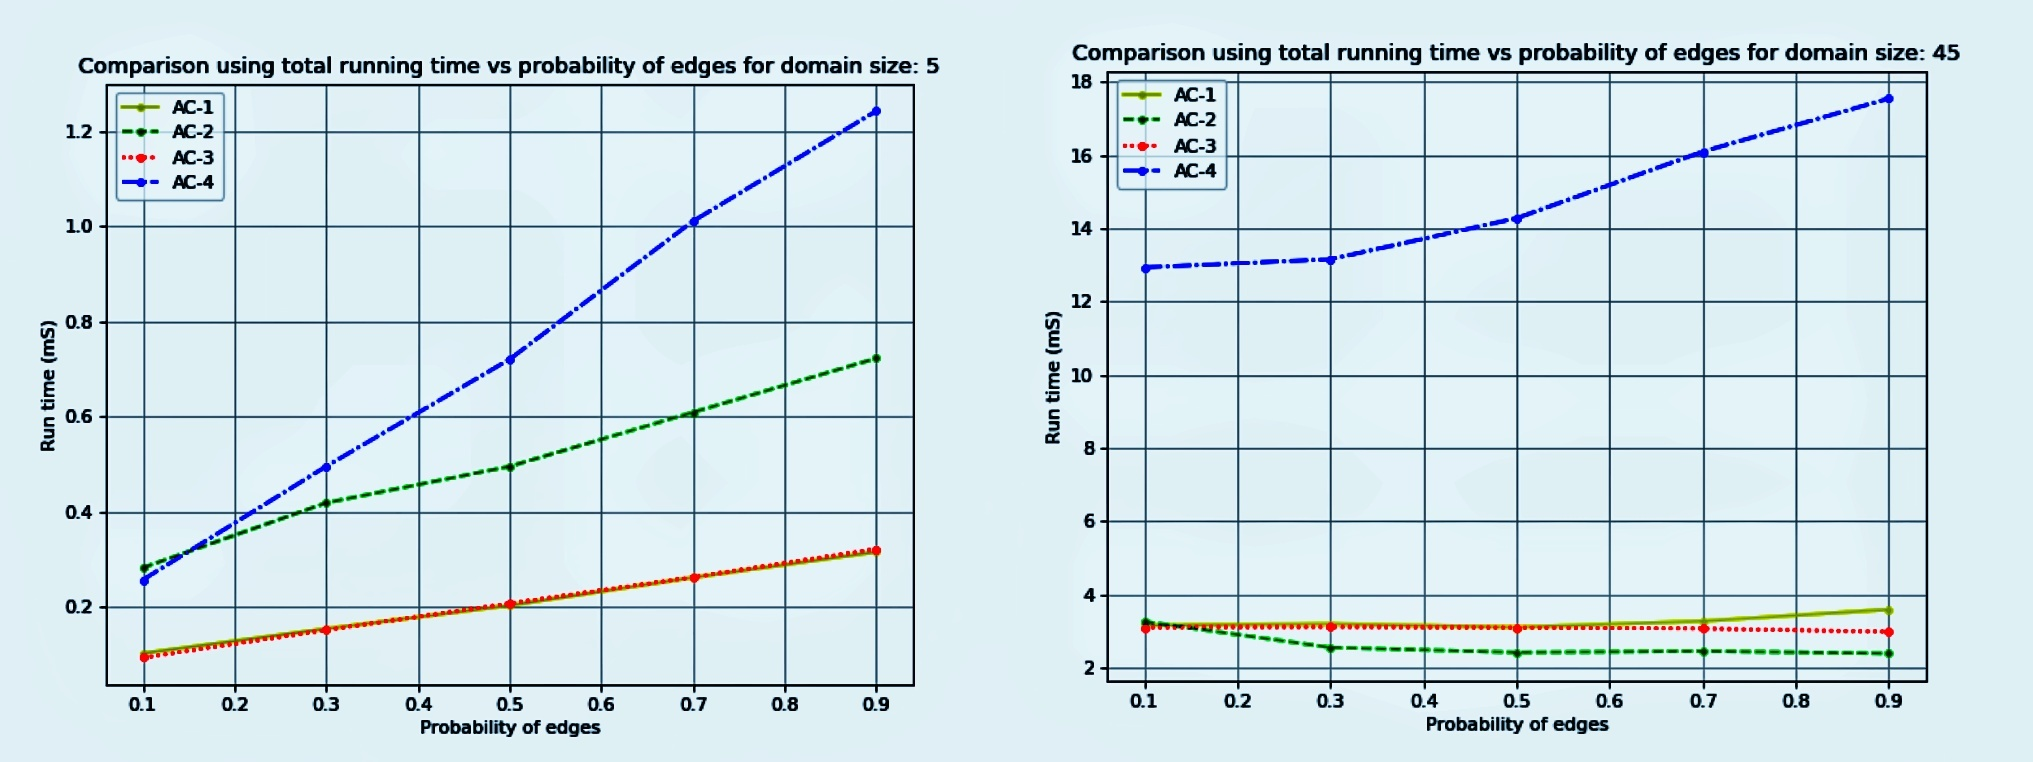
\includegraphics[width=\textwidth,height=2.6in]{44.jpeg}}
		{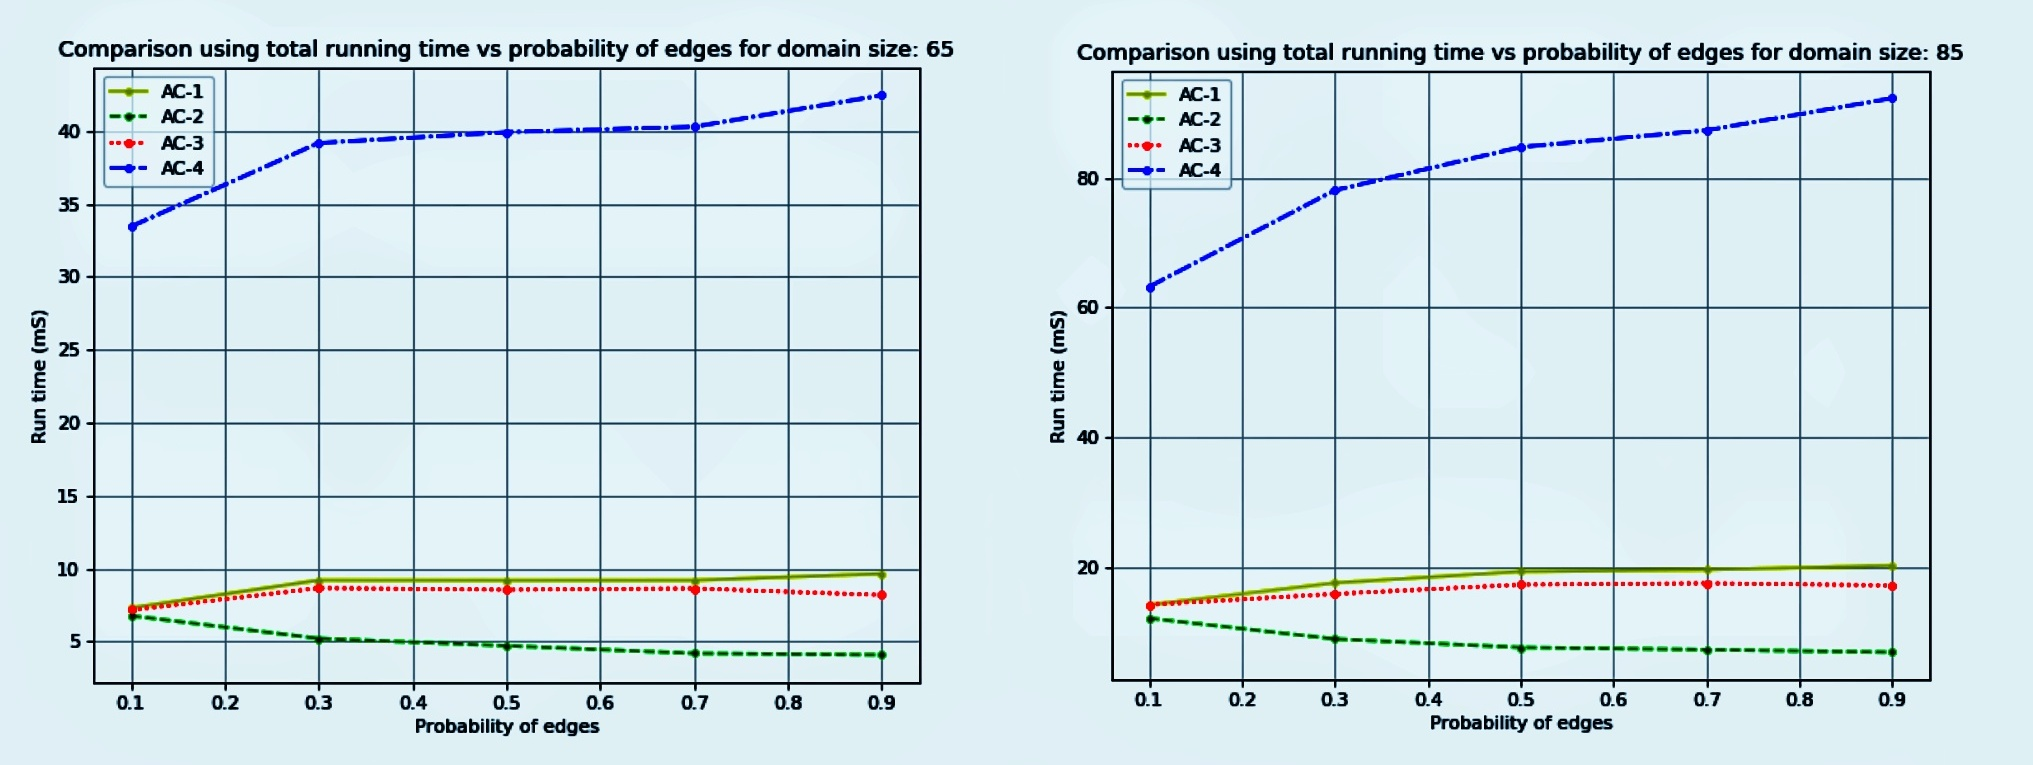
\includegraphics[width=\textwidth,height=2in]{33.jpeg}}
		\caption{\textbf{Probability of edges vs Run-time for domain size 5, 45, 65, 85}}
        \label{fig: 2}
\end{figure}

\section{\textit{Findings}}
\par
From the relative comparisons, it is clear that the performance of these four algorithms depends highly on \textit{domain size} as well as \textit{constraints selected}, \textit{number of nodes}, \textit{edges}, and other factors. From Figure 1, we can conclude that, for small domain size, performances are close to one another. Both \textbf{AC-1} and \textbf{AC-3} performs well in that case. But for larger domain size, \textbf{AC-2} performs best and \textbf{AC-4} worst. Running time increases dramatically for \textbf{AC-4} when we use larger domain size. \\\\
In Figure 2, conditions are very similar to that of Figure 1. Running time of \textbf{AC-4} increases dramatically and \textbf{AC-2} performs best for larger domains. The performance of \textbf{AC-1} and \textbf{AC-3} are very similar in this case. From these findings, we can conclude that \textbf{AC-2} is the best performer in my case. Although \textbf{AC-4} has the best run time \textit{(ek$^2$)} in the worst case scenario, in the best case, \textbf{AC-1} and \textbf{AC-3} outperform \textbf{AC-4}.



\end{document}
\grid